\subsection{Twitter Analysis}\label{sec:twitter-analysis}
Twitter is a global social media site with more than 328 million active users
\citep{SocialMediaStats}. Twitter's have two types of users, private citizens
and businesses. While businesses might use Twitter for announcements and
marketing, private citizens are more likely to use Twitter for general
communication and to discuss global and local events. In general, Twitter
defines itself as being used for the following purposes \citep{StartingTwitter}:

\begin{enumerate}    
  \item News and Politics.
  \item Sports.
  \item Pop Culture. 
  \item Influencers.
  \item Utility.
\end{enumerate} 

\begin{figure}[H] 
	\centering 
	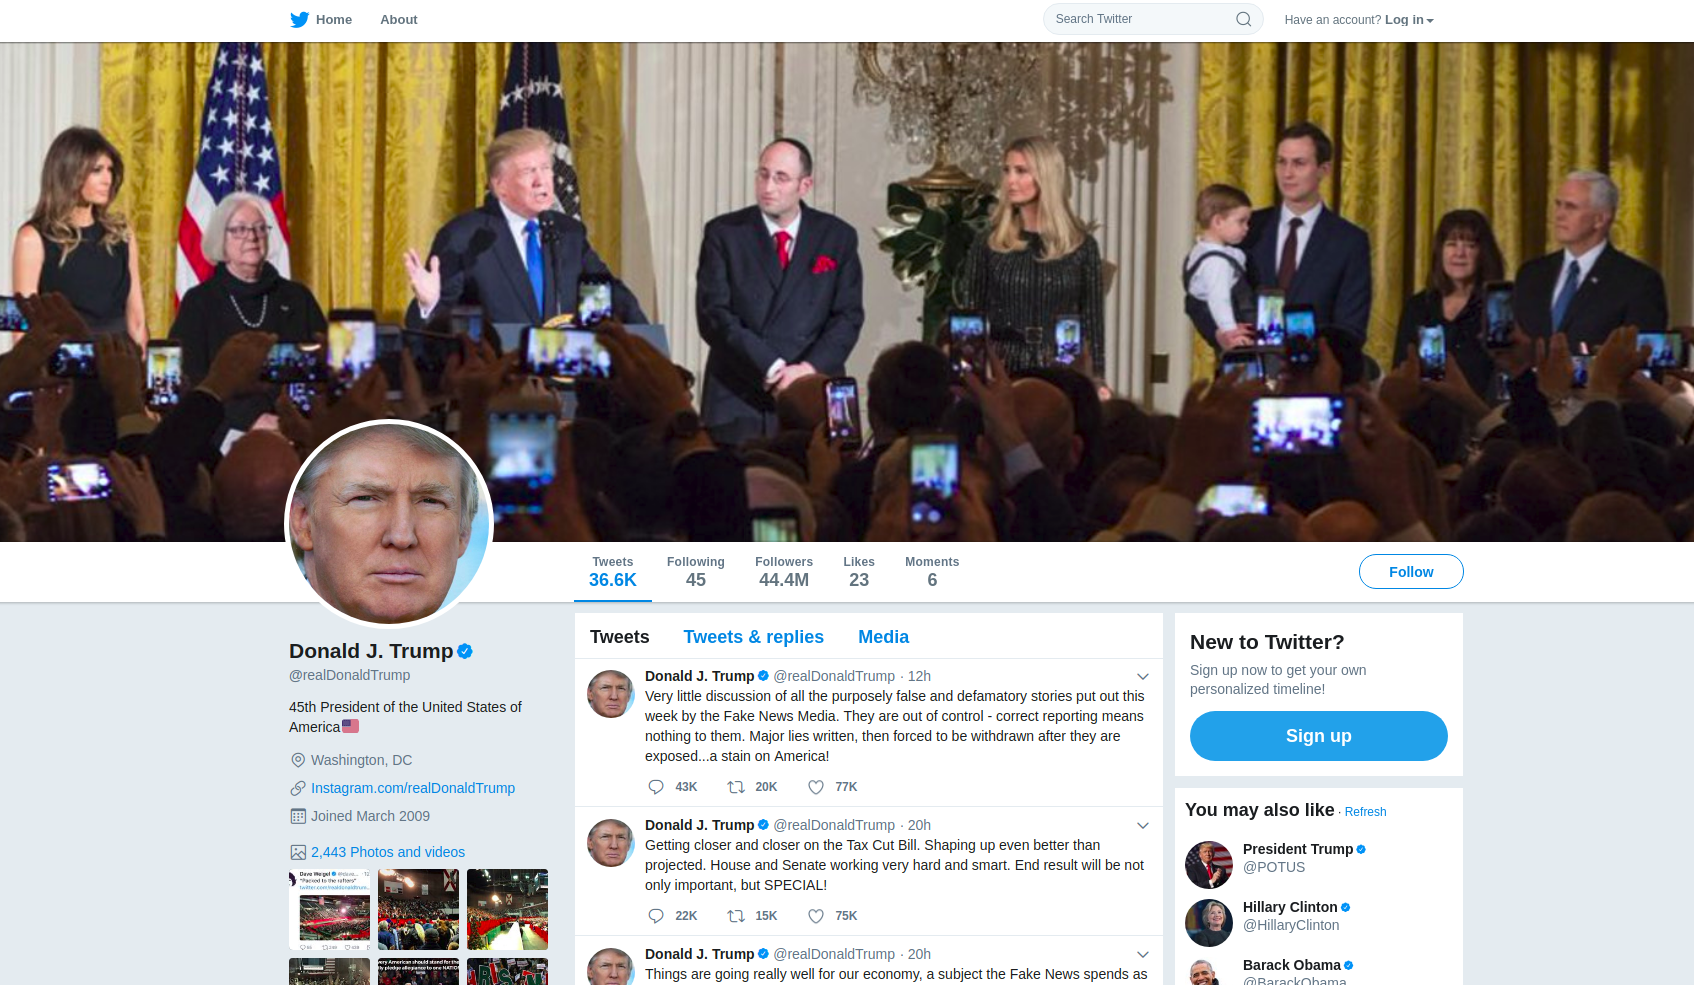
\includegraphics[width = 0.8\textwidth]{figures/DonDrumpf.png}
	\caption{Example of an ``influencers'' tweet from \@realDonaldTrump.}
	\label{fig:DrumpF}
\end{figure}]

\subsubsection{Using Twitter}
A Twitter user can make use of the following elements \citep{StartingTwitter}
in order to make tweets and communicate with other users:

\begin{itemize}
  \item \textbf{Tweet:} A tweet is a message, which a user can post from their
  account. A tweet can contain 280 characters \citep{Tweet280} of text, links,
  pictures and similar media sources, and be seen by all other users. Users who
  ``follow'' an account will automatically receive its tweet on their Twitter
  feed \citep{StartingTwitter2}.
  \item \textbf{Follow:} A user can choose to follow other peoples accounts,
  then they will get a notification whenever that account makes a tweet or
  retweets an existing tweet.
  \item \textbf{Retweet:} Instead of making a tweet, a user can forward a tweet
  made by another account. A user can choose to either retweet a tweet as it is,
  or embed the tweet into a tweet of their own. A user can make comments or
  remarks concerning the original tweet \fix{}{The last part,
  does the source not say}.
  \item \textbf{Hashtag:} When a user tweets or retweets, they can add a
  ``hashtag'', which can be used to group the tweet, with other tweets
  containing the same hashtag. Examples of hashtags usage on Twitter could be
  \#Politics or \#Sports, or to specify the user's opinion on a subject, e.g.
  \#war \#Idiotic. On Twitter hashtags are used for grouping, searching and
  filtering \fix{}{Much more than the source say}.
\end{itemize}

% \subsubsection{Tweet}
% A tweet is a message, which a user can post from their account. A tweet can
% contain 280 characters \citep{StartingTwitter2} \fix{}{That is not someting
% that source says} of text, links, pictures and similar media sources, and be
% seen by all other users. Users who ``follow'' the account will automatically be
% presented with the tweet on their Twitter feed.
% 
% \subsubsection{Follow}
% A user can choose to follow other peoples accounts. Then they will get a
% notification whenever a followed account makes a tweet or retweets an existing
% tweet.
% 
% \subsubsection{Retweet}
% Instead of making a tweet, a user can choose to forward a tweet made by another
% account. A user can either retweet the tweet as it is, or embed the tweet into a
% tweet of their own. A user can make comments or remarks in relation to the
% original tweet \fix{}{The last part, does the source not say}.
% 
% \subsubsection{Hashtag}
% When a user tweets or retweets, they can add a ``hashtag'', which can be used to
% group the tweet, with other tweets using the same hashtag. A hashtag is used as
% a general tag, such as \#Politics or \#Sports, or to specify the user's
% opinion on a subject e.g. \#war \#Idiotic. In general, hashtags are used for
% grouping, searching and filtering  \fix{}{Much more than the source say}.

\subsubsection{Twitter \acp{API}} \label{sub:twitterapi}
Twitter permits developers to retrieve data from their users, tweets and
trending hashtags. Twitter has three main \acp{API}, namely the \ac{REST}
\ac{API}, the Streaming \ac{API} and the Ads \ac{API} \citep{TwitterDevDocs}.
For this project, the \ac{REST} \ac{API} is the best fit, as it permits reading
Twitter' user data.

\subsubsection{REST API}
The \ac{REST} \ac{API} makes use of \ac{HTTP} requests to allow developers
access to Twitter's data \citep{TwitterREST}. Also, by using the OAuth protocol
\citep{TwitterOAuth}, Twitter enforce that only authorised applications can
access Twitter's data. All requests must be made using the \ac{HTTP} protocol.
These requests are structured differently based on the requested data.
\autoref{httpReq} shows an example of a \ac{HTTP} request with each part denoted
with a number and further explained in \autoref{httpReq}.

\figx{httpReq}{Structure of Twitter HTTP Request.}

\begin{table}[H] 
\begin{centering}
\begin{tabular}{|l|p{9cm}|l|}
\hline
\textbf{No}&	\textbf{Description}										\\\hline
1			&	Denotes the type of request: GET, POST, DELETE.				\\\hline
2			&	Address for the Twitter \ac{API}.							\\\hline
3			&	Name of the requested resource.	   							\\\hline
4			&	Format of the requested resource.							\\\hline
5			&	Index of the page of the requested data. In case all data can not be
retrieved in a single page.													\\\hline 
6			&	Extra parameters such as the name of the requested user.	\\\hline
7			&	Number of data points requested. Maximum of 5000 per page.	\\\hline
\end{tabular}
\caption{Elaboration on the Twitter HTTP requests.}
\label{httpElaboration}
\end{centering}
\end{table}
